% \pagebreak[4]
% \hspace*{1cm}
% \pagebreak[4]
% \hspace*{1cm}
% \pagebreak[4]

\chapter{Segundo Capítulo}
\graphicspath{{Chapters/Chapter1/Chapter1Figs/PNG/}{Chapters/Chapter1/Chapter1Figs/PDF/}{Chapters/Chapter1/Chapter1Figs/}}

\section{Primeiro Parágrafo}
Agora começo com o meu primeiro parágrafo aqui... com uma nota de rodapé \footnote{nota de rodapé}.


Segue-se uma equação :
\begin{eqnarray}
CIF: \hspace*{5mm}F_0^j(a) &=& \frac{1}{2\pi \iota} \oint_{\gamma} \frac{F_0^j(z)}{z - a} dz
\end{eqnarray}


\section{Segundo Parágrafo}
e aqui posso escrever mais ... \cite{texbook}

\subsection{Primeiro sub-parágrafo}
... e mais ...
agora posso citar individualmente : \cite{latex} e \cite{texbook}
e \cite{Rud73}; ou agrupando : \cite{latex, texbook, Rud73}.

Vou agora incluir uma imagem :
\begin{figure}[!htbp]
  \begin{center}
    \leavevmode
    \ifpdf
      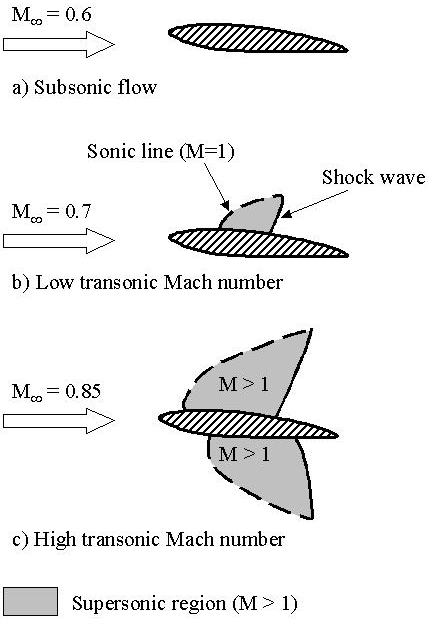
\includegraphics[height=6in]{aflow}
    \fi
    \caption{Legenda}
    \label{FigAir}
  \end{center}
\end{figure}

Posso colocar uma referência cruzada no texto desta forma (\ref{FigAir}) e esta referência cruzada encontra-se na página \pageref{FigAir}. 

